\documentclass[11pt]{exam}
\usepackage[a4paper,width=170mm,top=10mm,bottom=18mm]{geometry}
%\usepackage[top=1in, bottom=1.25in, left=1.25in, right=1.25in]{geometry}
\usepackage{graphicx,lastpage}
\usepackage{upgreek}
\usepackage{censor}
\usepackage{tabularx}
\usepackage{xcolor}
\usepackage{amsmath}
%\usepackage{cleveref}
%\usepackage{tabularx,pbox}
%\usepackage[nopar]{lipsum}
\usepackage{longtable}
\usepackage{multirow}
\usepackage[inline]{enumitem}
\usepackage{float}
\usepackage{tikz}
\usepackage{boldline}
\usepackage{amssymb}
\usepackage{pdfrender}
\usepackage{pgfplots}  
\pgfplotsset{width=10cm,compat=1.8} 
\def\checkmark{\tikz\fill[scale=0.4](0,.35) -- (.25,0) -- (1,.7) -- (.25,.15) -- cycle;} 
\setlength{\parindent}{0pt}
\definecolor{blue(pigment)}{rgb}{0.2, 0.2, 0.6}
\flushbottom
\usepackage[normalem]{ulem}
\renewcommand{\thesection}{\large \Roman{section}}
\pagestyle{headandfoot}
\usepackage{dcolumn}
\usepackage{colortbl}

\begin{document}

%==============================================================
	\begin{minipage}{\linewidth}
	\begin{minipage}{0.14\linewidth}%
		
\includegraphics[width=0.85\textwidth]{logo.png}\end{minipage}
	\begin{minipage}[r]{0.86\textwidth}%
		\noindent
		\begin{center}	
			\renewcommand{\arraystretch}{1.0}
			\textcolor{blue}{\Large \bfseries INSTITUTE OF AERONAUTICAL ENGINEERING}\\
			%\hspace*{5.2cm} 
			\textcolor{blue}{\Large (Autonomous)} \\
			%\hspace*{4.7cm}
			\small Dundigal, Hyderabad - 500 043 \\  [3pt] 
			\large \bfseries AERONAUTICAL ENGINEERING \\\vspace{2pt}
	\textcolor{red}{\large \bfseries COURSE DESCRIPTION} \\\vspace{3pt}
\end{center}
\end{minipage}\end{minipage}
\par
\newcolumntype{C}[1]{>{\centering\arraybackslash}p{#1}}
\newcolumntype{R}[1]{>{\raggedright\arraybackslash}p{#1}}
\renewcommand{\arraystretch}{1.2}
%\vspace{0.5cm}
\begin{flushleft}
	\begin{tabular}{|R{5cm}|R{3.5cm}|l|c|c|c|}
	\hline
	Course Title                      & \multicolumn{5}{l|}{ \textbf{AEROSPACE STRUCTURAL DYNAMICS}}                                                                  \\ \hline
	Course Code                       & \multicolumn{5}{l|}{AAEC35}                                                                              \\ \hline
	Program                           & \multicolumn{5}{l|}{B.Tech}                                                                              \\ \hline
	Semester                          & VII                         & \multicolumn{4}{l|}{AE}                                                   \\ \hline
	Course Type                       & Core                     & \multicolumn{4}{l|}{}                                                     \\ \hline
	Regulation                        & IARE                   & \multicolumn{4}{l|}{UG-20}                                                     \\ \hline
	\multirow{3}{*}{Course Structure} & \multicolumn{3}{c|}{Theory}                                             & \multicolumn{2}{c|}{Practical} \\ \cline{2-6} 
	& \multicolumn{1}{c|}{Lecture} & \multicolumn{1}{c|}{Tutorials} & Credits & Laboratory      & Credits      \\ \cline{2-6} 
	& \multicolumn{1}{c|}{3}       & 1                              & 4       & -               & -            \\ \hline
	Course Coordinator                 & \multicolumn{5}{l|}{Mr. K Arun Kumar, Assistant Professor}                                          \\ \hline
\end{tabular}
\end{flushleft}
\vspace{-0.75cm}
\begin{flushleft}
\textcolor{blue}{\section{\large \bfseries COURSE PRE-REQUISITES:}}\vspace{-0.25cm}
\begin{tabular}{|>{\centering\arraybackslash}p{2cm}  | >{\centering\arraybackslash}p{4cm}  |   >{\centering\arraybackslash}p{2.2cm} |>{\centering\arraybackslash}p{7cm}|} 
	\hline 		
	\textbf{Level}&	\textbf{Course Code}&	\textbf{Semester}&	\textbf{Prerequisites}\\ 
	\hline
	B.Tech&	AHSC03&	I&Engineering Physics\\ 
	\hline
	B.Tech&	AMEC01&	II&Engineering Mechanics\\ 
	\hline
	B.Tech&	AAEC01&	III&Mechanics of Solids\\ 
	\hline
\end{tabular}\end{flushleft}

\textcolor{blue}{\section{\large \bfseries COURSE OVERVIEW:}}\vspace{-0.25cm}
The Mechanical Systems as well as Mechanical Structures often experience various periodic Vibrations when they are used in their physical state. These Vibrations have both advantages and disadvantages to the machinery. This course Aims to teach how to address these vibrations by converting the physical models into mathematical models, solving those models using mathematical techniques and then interpreting the results in a physical Context. Additionally, the course also offers introductory to both theoretical and experimental principles of aeroelasticity.
 
\vspace{-0.65cm}
\begin{flushleft}
\textcolor{blue}{\section{\large \bfseries MARKS DISTRIBUTION:}}
	\begin{tabular}{|>{\centering\arraybackslash}p{3.5cm}  | >{\centering\arraybackslash}p{5.75cm}  |   >{\centering\arraybackslash}p{3.5cm} |>{\centering\arraybackslash}p{2.4cm}|}
		\hline 
	\textbf{Subject}&	\textbf{SEE Examination}&	\textbf{CIE Examination}&	\textbf{Total Marks}\\ 
	\hline
	Aerospace Structural Dynamics&70 Marks&30 Marks&100\\ 
	\hline
	\end{tabular}
\end{flushleft}\vspace{-0.75cm}
\begin{flushleft}
\textcolor{blue}{\section{\large \bfseries DELIVERY / INSTRUCTIONAL METHODOLOGIES:}}
	\begin{tabular}{|>{\centering\arraybackslash}p{0.3cm}  | >{\centering\arraybackslash}p{4.3cm}  |   >{\centering\arraybackslash}p{0.5cm} |>{\centering\arraybackslash}p{2.6cm}|>{\centering\arraybackslash}p{0.5cm}  | >{\centering\arraybackslash}p{2.5cm}  |   >{\centering\arraybackslash}p{0.5cm} |>{\centering\arraybackslash}p{2.2cm}|}
	\hline 

\checkmark &  PPT   & \checkmark& Chalk \& Talk  & \centering \checkmark &Assignments  & \textbf{x} & MOOC \\ \hline
\checkmark & Open Ended Experiments   & \textbf{x}  & Seminars  & \textbf{x} & Mini Project & \checkmark &Videos  \\ \hline
\end{tabular}
\end{flushleft}

\textcolor{blue}{\section{\large \bfseries EVALUATION METHODOLOGY:}}\vspace{-0.25cm}
The course will be evaluated for a total of 100 marks, with 30 marks for Continuous Internal Assessment (CIA) and 70 marks for Semester End Examination (SEE).  CIA  is  conducted for a total of 30 marks, with 20 marks for Continuous Internal Examination (CIE),  and 10 marks for Alternative Assessment Tool (AAT).\\

\textbf{Semester End Examination (SEE):} The SEE is conducted for 70 marks of 3 hours duration. The syllabus for the theory courses is divided into FIVE modules and each module carries equal weightage in terms of marks distribution. The question paper pattern is as follows. Two full questions with "either" or "choice" will be drawn from each module. Each question carries 14 marks. There could be a maximum of two sub divisions in a question.\\
The expected percentage of cognitive level of the questions is broadly based on the criteria given in below Table.
\begin{longtable}{|C{8cm}|C{8cm}|}
	\hline
     Percentage of Cognitive Level&	Blooms Taxonomy Level\\\hline
	10\%&	Remember\\\hline
35\%&	Understand\\\hline
	55\%&	Apply\\\hline

\end{longtable}
\large \textbf{Continuous Internal Assessment (CIA):}\\
CIA is conducted for a total of 30 marks, with 20 marks for continuous internal examination (CIE) and 10 marks for Alternative Assessment Tool (AAT).
\begin{longtable}{|>{\centering\arraybackslash}p{1.5cm}  | >{\raggedright\arraybackslash}p{9cm}  |   >{\centering\arraybackslash}p{2.2cm} |>{\centering\arraybackslash}p{2.4cm}  |}
	\hline
	\multicolumn{2}{|c|}{\textbf{Component}}                                          & Marks  &        Total Marks            \\ \hline
	\multicolumn{1}{|c|}{\multirow{4}{*}{\textbf{CIA}}} & Continuous Internal Examination – 1 (Mid-term)  &10  & \multirow{4}{*}{30} \\ \cline{2-3}
	& Continuous Internal Examination – 2 (Mid-term) & 10 &                   \\ \cline{2-3}
	& AAT-1 & 5 &                   \\ \cline{2-3}
	& AAT-2 &  5&                   \\ \hline
	\textbf{SEE }   & Semester End Examination (SEE) & 70 &     70              \\ \hline
	\multicolumn{3}{|c|}{\textbf{Total Marks}}                                             &           100        \\ \hline
\end{longtable}

\textbf{Continuous Internal Examination (CIE):}\\
Two CIE exams shall be conducted at the end of the $8^{th}$ and $16^{th}$ week of the semester respectively for 10 
marks  each  of  2  hours  duration  consisting  of  five  descriptive  type  questions  out  of  which  four  questions 
have  to  be  answered.

\vspace{0.5cm}
\textbf{Alternative Assessment Tool (AAT)}\\
This AAT enables faculty to design own assessment patterns during the CIA. The AAT converts the classroom into an effective learning center. The AAT may include tutorial hours/classes, seminars, assignments, term paper, open ended experiments, METE (Modeling and Experimental Tools in Engineering), five minutes video, MOOCs etc. The AAT chosen for this course is given in below table
\begin{longtable}{|>{\centering\arraybackslash}p{5.2cm}  | >{\centering\arraybackslash}p{5.2cm}  |   >{\centering\arraybackslash}p{5cm} |}
	\hline
	AAT-II&	Tech-talk&	Complex Problem Solving\\ \hline
	40\%&	40\%&	20\%                 \\ \hline
\end{longtable}\vspace{-0.6cm}		
\textcolor{blue}{\section{\large \bfseries COURSE OBJECTIVES:}}
\vspace{-0.3cm}		
\textbf{The students will try to:}
\vspace{-0.25cm}
\newcolumntype{C}[1]{>{\centering\arraybackslash}p{#1}}
\newcolumntype{R}[1]{>{\raggedright\arraybackslash}p{#1}}
\renewcommand{\arraystretch}{1.2}
\begin{flushleft}	
	\begin{longtable}{|C{1.5cm}|R{15cm}|}
		\hline
		I &  Using the newton's 2nd law of motion and energy principles develop the mathematical models for the problems in vibrations.\tabularnewline
		\hline
		II & Figure out a comprehensive solution to the modeled mechanical vibration problems.
	\tabularnewline
		\hline
		III &    Develop a new mechanical system which has desirable vibrational behavior.\tabularnewline
		\hline	
		IV & Evaluate the underlying assumptions in the aeroelastic analysis of fixed-wing and rotary-wing aerospace vehicles and systems.
	\tabularnewline
		\hline
	\end{longtable}
\end{flushleft}\vspace{-1.5cm}

\textcolor{blue}{\section{\large \bfseries COURSE OUTCOMES:}}
\vspace{-0.3cm}	
\textbf{After successful completion of the course, students should be able to:}\\
\renewcommand{\arraystretch}{1.1}\vspace{-0.75cm}
\begin{flushleft}
	\begin{longtable}{|C{1.5cm}|R{12.5cm}|C{2cm}|}
		\hline
		CO 1 &	\textbf{Apply} \textcolor{blue}{ newton's second law of motion and the principle of conservation of energy with various principles of mechanical vibrations  to the mathematical models  } \textcolor{red}{for obtaining
			their governing equations of motion.}&Apply\tabularnewline
		\hline
		CO 2&	\textbf{Generate} \textcolor{blue}{   the two degrees of
			freedom systems the mathematical modeling } \textcolor{red}{ for determining the frequency of spring-mass system.}&	Analyze\tabularnewline
		\hline
		CO 3&	\textbf{Relate} \textcolor{blue}{ mode shapes and  the natural frequencies   of a multi	degree of freedom system } \textcolor{red}{ for distributing parameter systems for the numerical solution }&	Apply\tabularnewline
		\hline 
	
		CO 4&	\textbf{Compute} \textcolor{blue}{  various numerical and theoretical  procedures } \textcolor{red}{for predicting the dynamic response of  continuous structural systems under most diverse loading conditions}.	&Apply\tabularnewline
		\hline		
		CO 5&\textbf{Construct } \textcolor{blue}{ solutions to the static aeroelasticity problems such as typical section and wing divergence
			problems; }\textcolor{red}{ for their selection in real world
			applications.}	&	Apply\tabularnewline
		
		
		\hline
	\end{longtable}
\end{flushleft}

\textbf{\textcolor{blue}{\large COURSE KNOWLEDGE COMPETENCY LEVEL}}
\begin{center}	
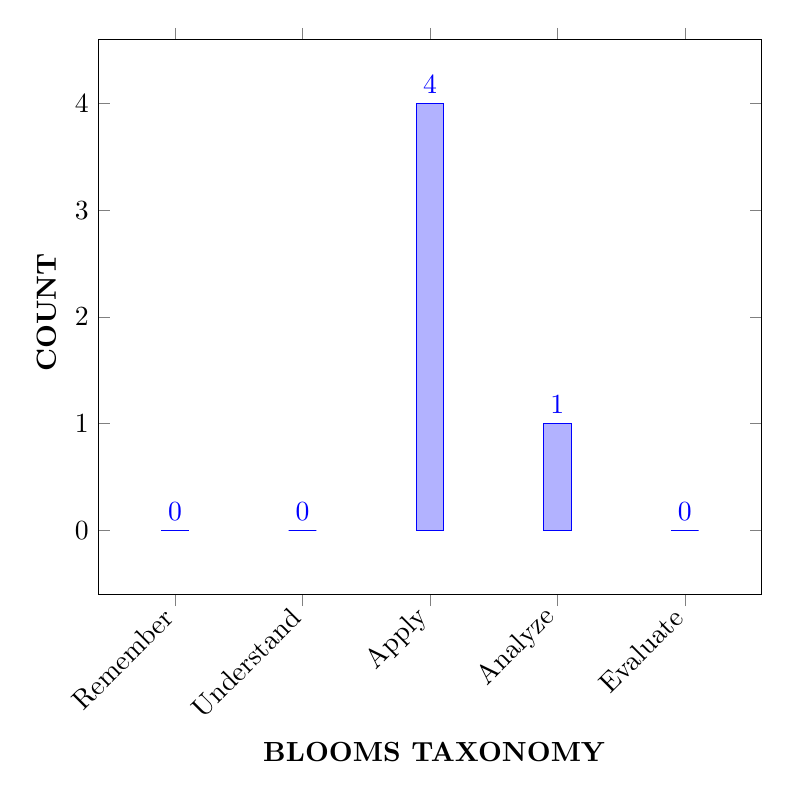
\begin{tikzpicture}  
\begin{axis}  [
ybar,
enlargelimits=0.15,
legend style={at={(0.5,-0.2)},
	anchor=north,legend columns=-1},
ylabel={\ \textbf{COUNT} },
xlabel={\ \textbf{BLOOMS TAXONOMY}},
symbolic x coords={Remember,Understand,Apply,%
	Analyze,Evaluate},
xtick=data,
nodes near coords,
nodes near coords align={vertical},
x tick label style={rotate=45,anchor=east},
]
\addplot coordinates {
	(Remember,0) (Understand,0) (Apply,4)
	(Analyze,1) (Evaluate,0)
};
\end{axis}  
\end{tikzpicture}
\end{center}
\newpage
\textcolor{blue}{\section{\large \bfseries  PROGRAM OUTCOMES: }}\vspace{-0.5cm}
\begin{flushleft}
	\begin{longtable}{|>{\centering\arraybackslash}p{1.6cm}  | >{\raggedright\arraybackslash}p{14cm}  | }
		\hline
		\multicolumn{2}{|c|}{\textbf{Program Outcomes}}  \\ \hline
		\endhead
		\hline
		PO 1&	\textbf{Engineering knowledge:} Apply the knowledge of mathematics, science, engineering fundamentals, and an engineering specialization to the solution of complex engineering problems.\\ \hline
		PO 2&	\textbf{Problem analysis:} Identify, formulate, review research literature, and analyze complex engineering problems reaching substantiated conclusions using first principles of mathematics, natural sciences, and engineering sciences.\\ \hline
		PO 3&	\textbf{Design/Development of Solutions:} Design solutions for complex Engineering problems and design system components or processes that meet the specified needs with  appropriate consideration for the public health and safety,
		and the cultural, societal, and Environmental considerations\\ \hline
		PO 4&	\textbf{Conduct Investigations of Complex Problems:} Use research-based knowledge and research methods including design of experiments, analysis and interpretation of data, and synthesis of the information to provide valid conclusions.\\ \hline
		PO 5&	\textbf{Modern Tool Usage: }Create, select, and apply appropriate techniques, resources, and modern Engineering and IT tools including prediction and modelling to complex Engineering activities with an understanding of the limitations\\ \hline
		
		PO 6& \textbf{The  engineer  and  society:} Apply reasoning informed by the contextual knowledge to assess 
		societal,  health,  safety,  legal  and  cultural  issues  and  the  consequent  responsibilities  relevant  to 
		the professional engineering practice. \\ \hline
		PO 7&  \textbf{Environment  and  sustainability:}  Understand  the  impact  of  the  professional  engineering 
		solutions  in  societal  and  environmental  contexts,  and  demonstrate  the  knowledge  of,  and  need 
		for sustainable development. \\ \hline
		PO 8& \textbf{Ethics:}  Apply  ethical  principles  and  commit  to  professional  ethics  and  responsibilities  and 
		norms of the engineering practice. \\ \hline
		PO 9& \textbf{Individual and team work:} Function effectively as an individual, and as a member or leader 
		in diverse teams, and in multidisciplinary settings. \\ \hline
		PO 10&  \textbf{Communication: } Communicate  effectively  on  complex  engineering  activities  with  the 
		engineering  community  and  with  society  at  large,  such  as,  being  able  to  comprehend  and  write 
		effective  reports  and  design  documentation,  make  effective  presentations,  and  give  and  receive 
		clear instructions. \\ \hline
		PO 11&  \textbf{Project management  and  finance: } Demonstrate  knowledge  and  understanding  of  the 
		engineering  and  management  principles  and  apply  these  to  one’s  own  work,  as  a  member  and 
		leader in a team, to manage projects and in multidisciplinary environments. \\ \hline
		PO 12&	\textbf{Life-Long Learning:} Recognize the need for and having the preparation and ability to engage in independent and life-long learning in the broadest context of technological change\\ \hline
	\end{longtable}
\end{flushleft}\newpage
%\vspace{-0.5cm}
\textcolor{blue}{\section{\large \bfseries HOW PROGRAM OUTCOMES ARE ASSESSED:}}
\begin{flushleft}
	\begin{longtable}{|>{\centering\arraybackslash}p{1.6cm}  | >{\raggedright\arraybackslash}p{9.2cm}  |   >{\centering\arraybackslash}p{1.8cm} |>{\centering\arraybackslash}p{3cm}|}
		\hline
		\multicolumn{2}{|c|}{\textbf{Program}} & \textbf{Strength} & \textbf{Proficiency Assessed by} \\ \hline
	PO 1&	\textbf{Engineering knowledge:} Apply the knowledge of mathematics, science, engineering fundamentals, and an engineering specialization to the solution of complex engineering problems.&	3&	CIE/Quiz/AAT\\ \hline
	PO 2&	\textbf{Problem analysis:} Identify, formulate, review research literature, and analyze complex engineering problems reaching substantiated conclusions using first principles of mathematics, natural sciences, and engineering sciences.&	3&	CIE/Quiz/AAT\\ \hline
	PO 3&	\textbf{Design/Development of Solutions:} Design solutions for complex Engineering problems and design system components or processes that meet the specified needs with  appropriate consideration for the public health and safety,
	and the cultural, societal, and Environmental considerations&	3&	CIE/Quiz/AAT\\ \hline
	\multicolumn{4}{l}{\textbf{3 = High; 2 = Medium; 1 = Low}}\\ 
			\end{longtable}
	\end{flushleft}\vspace{-2cm}
\textcolor{blue}{\section{\large \bfseries HOW PROGRAM SPECIFIC OUTCOMES ARE ASSESSED:}}
\begin{flushleft}
	\begin{longtable}{|>{\centering\arraybackslash}p{1.8cm}  | >{\raggedright\arraybackslash}p{9cm}  |   >{\centering\arraybackslash}p{2cm} |>{\centering\arraybackslash}p{2.6cm}|}
		\hline
		\multicolumn{2}{|c|}{\textbf{Program}} & \textbf{Strength} & \textbf{Proficiency Assessed by} \\ \hline
	
		PSO 2&	Focus on formulation and evaluation of aircraft
		elastic bodies for characterization of aero elastic
		phenomena. &	2&	Quiz\\ \hline

		\multicolumn{4}{l}{\textbf{3 = High; 2 = Medium; 1 = Low}}\\ 
		\end{longtable}
\end{flushleft}\vspace{-2cm}
\textcolor{blue}{\section{\large \bfseries MAPPING OF EACH CO WITH PO(s),PSO(s):}}
\begin{flushleft}
	\begin{longtable}{|>{\centering\arraybackslash}p{2.2cm}  | >{\centering\arraybackslash}p{0.5cm}  |   >{\centering\arraybackslash}p{0.5cm} |>{\centering\arraybackslash}p{0.5cm}|>{\centering\arraybackslash}p{0.5cm}  | >{\centering\arraybackslash}p{0.5cm}  |   >{\centering\arraybackslash}p{0.5cm} |>{\centering\arraybackslash}p{0.5cm}|>{\centering\arraybackslash}p{0.5cm}  | >{\centering\arraybackslash}p{0.5cm}  |   >{\centering\arraybackslash}p{0.5cm} |>{\centering\arraybackslash}p{0.5cm}|>{\centering\arraybackslash}p{0.5cm}  V{5.5} >{\centering\arraybackslash}p{0.65cm}  |   >{\centering\arraybackslash}p{0.65cm} |>{\centering\arraybackslash}p{0.65cm}|}
		\hline
		\multirow{2}{*}{\textbf{\begin{tabular}[c]{@{}c@{}}\\\small  COURSE \\\small OUTCOMES\end{tabular}}} & \multicolumn{12}{cV{5.5}}{\textbf{PROGRAM OUTCOMES}}  & \multicolumn{3}{c|}{\textbf{\begin{tabular}[c]{@{}c@{}}\small PSO'S \end{tabular}}} \\ \cline{2-16} 
		& PO 1 & PO 2 &PO 3 & PO 4 & PO 5 & PO 6 & PO 7 & PO 8 & PO 9 & PO 10 & PO 11 & PO 12 &PSO 1              & PSO 2              & PSO 3              \\ 
		\hline
		\endhead
CO 1   & \checkmark  & \checkmark & -  &  - &  - &  - & -  & -  &  - &-   &  -  &    &        -                             &         \checkmark                    &  -                                   \\ \hline
CO 2   &  \checkmark &  \checkmark & -  &  - &  - & -  &  - & -  &  - &  -  &  -  & -   &                                    &        \checkmark                     &   -                                  \\ \hline
CO 3   &\checkmark   &  \checkmark  &  - & -  &  - &   -& -  & -  &  - &  -  &  -  & -   &                                &                \checkmark                  &     -                                \\ \hline
CO 4   & \checkmark  &  \checkmark & -  &  - & - &   -& -  &  - & -  &  -  &   - &    &                                  &\checkmark                                     &        -                             \\ \hline
CO 5   & \checkmark  &\checkmark  & -  &  - &  - &  - & - &  - & -  &   - & -   &  -  &                         -            &         \checkmark                       &  -                                   \\ \hline

			\end{longtable}
	\end{flushleft}
\vspace{-2cm}
\newpage
\textcolor{blue}{\section{\large \bfseries JUSTIFICATIONS FOR CO – (PO, PSO) MAPPING -DIRECT:}}
\renewcommand{\arraystretch}{1.2}
\begin{flushleft}
	\begin{longtable}{|>{\centering\arraybackslash}p{1.8cm}  | >{\centering\arraybackslash}p{1.2cm}  |   >{\raggedright\arraybackslash}p{10cm} |>{\centering\arraybackslash}p{2cm}|} 
		\hline
			
		\tiny \textbf{\begin{tabular}[c]{@{}c@{}}\tiny COURSE \\\tiny OUTCOMES\end{tabular}} &\textbf{\begin{tabular}[c]{@{}c@{}}\tiny PO'S \\\tiny PSO'S\end{tabular}}   & \small \textbf{Justification for mapping (Students will be able to)}                                                                                                                                                                                                                                                                                                                                                                                                                                                                                                    &\tiny \textbf{\begin{tabular}[c]{@{}c@{}}\tiny No. of Key \\\tiny Competencies\end{tabular}}  \\ 
		
		\hline
		\endhead
		 CO 1&	PO 1&Understand the concepts of the equation of motion of free vibration and its response for determining the nature of single degree of freedom  using the knowledge of \textbf {mathematics, science and Engineering fundamentals.} &	3\\\cline{2-4}
		 &PO 2& Identify the formula to simplify the harmonnic
		 response problems on free vibration by using
		 mathematics and engineering knowledge.&
		 2\\\cline{2-4}
		 &PSO 2& Apply the equation of free vibration system for the
		 solving of the undamped system using engineering
		 fundamentals.&
		 1\\\hline
		CO 2&	PO 1&	Explain various equations of forced vibration for
		identifying the frequency of the vibrating system by
		applying the \textbf{principles of mathematics, science and
		engineering fundamentals.}&	3\\\cline{2-4}
		&PO 2&	Understand the given \textbf{problem statement and
		formulate} variation of phase angle across different
		waves by the \textbf{provided information and data} in
		reaching substantiated conclusions by the
		interpretation of results.
 &	2\\\cline{2-4}
&PSO 2& Use the equation of free and forces vibrating system for
the solving of the damped and undamped system by
using mathematics, science and Engineering
fundamentals.&
1
\\\hline
		CO 3&	PO 1&	Understand the torsional vibrations of rotor and
		geared systems for determining the DOF of the
		vibrating systems based on \textbf{mathematical principles
		and engineering fundamentals }of vibrations. &	3\\\cline{2-4}
      &	PO 2&	Identify the formula to simplify the torsional vibrations
      of rotor and geared systems by \textbf{using mathematics
      and engineering knowledge. } &	2\\\cline{2-4}  
 &	PSO 2&	Use the equation of multi degree of freedom vibrating
 system for simplifying the complex problems using
 engineering fundamentals. &	1\\\hline
		CO 4&	PO 1&	Develop the governing equations for a multi degree of
		freedom vibrating system by applying the principles of
		\textbf{mathematics, science and Engineering
		fundamentals.} &	3\\\cline{2-4}
      &	PO 2&Identify the formula of stiffness and flexibility influence
      coefficients for simplifying solutions of multi DOF
      systems by using \textbf{mathematics and engineering
      knowledge} &	2\\\cline{2-4} \hline 
 &	PSO 2&	Apply the equation of free vibrating system for the
 solving of the damped and damped system using
\textbf{ mathematics, science and Engineering
 fundamentals.} &	1\\\hline
		CO 5&	PO 1&	Understand the concepts of the vibration for
		determining the frequency of cable, rod, shaft by using
		the knowledge of \textbf{mathematics, science and
		Engineering fundamentals.} &	3\\\cline{2-4} 
	&	PO 2&Apply the given \textbf{problem statement and formulate}
	transverse, longitudinal, torsional and lateral
	vibrations of cables, rods and beams information and
	data in reaching substantiated conclusions by the
	interpretation of results. &	2\\\cline{2-4}  
	&	PSO 2&	Analyse the frequency of cable, shafts, beam for
	developing the new solutions on vibrating body using
	\textbf{appropriate mathematics, science and engineering
	fundamentals.} &	1\\\hline

			
	\end{longtable}	
\end{flushleft}
\vspace{-1cm}
\textcolor{blue}{\section{\large \bfseries TOTAL COUNT OF KEY COMPETENCIES FOR CO – (PO, PSO) MAPPING:}}
\vspace{-0.2cm}
\begin{flushleft}
	\begin{longtable}{|>{\centering\arraybackslash}p{2.2cm}  | >{\centering\arraybackslash}p{0.5cm}  |   >{\centering\arraybackslash}p{0.5cm} |>{\centering\arraybackslash}p{0.5cm}|>{\centering\arraybackslash}p{0.5cm}  | >{\centering\arraybackslash}p{0.5cm}  |   >{\centering\arraybackslash}p{0.5cm} |>{\centering\arraybackslash}p{0.5cm}|>{\centering\arraybackslash}p{0.5cm}  | >{\centering\arraybackslash}p{0.5cm}  |   >{\centering\arraybackslash}p{0.5cm} |>{\centering\arraybackslash}p{0.5cm}|>{\centering\arraybackslash}p{0.5cm}  V{5.5} >{\centering\arraybackslash}p{0.65cm}  |   >{\centering\arraybackslash}p{0.65cm} |>{\centering\arraybackslash}p{0.65cm}|}
		\hline
		\multirow{2}{*}{\textbf{\begin{tabular}[c]{@{}c@{}}\\\small  COURSE \\\small OUTCOMES\end{tabular}}} & \multicolumn{12}{cV{5.5}}{\textbf{PROGRAM OUTCOMES}}  & \multicolumn{3}{c|}{\textbf{\begin{tabular}[c]{@{}c@{}}\small PSO'S \end{tabular}}} \\ \cline{2-16} 
		& PO 1 & PO 2 &PO 3 & PO 4 & PO 5 & PO 6 & PO 7 & PO 8 & PO 9 & PO 10 & PO 11 & PO 12 &PSO 1              & PSO 2              & PSO 3              \\ 
		\hline
		\endhead
		CO 1   & 3  &2 & -  &  - &  - &  - & -  & -  &  - &-   &  -  &  -  &        -                             &         1                           &  -                                   \\ \hline
		CO 2   &  2 & 3 & -  &  - &  - & -  &  - & -  &  - &  -  &  -  & -   &         -                            &        1                             &   -                                  \\ \hline
		CO 3   &3   &  2 &  - & -  &  - &   -& -  & -  &  - &  -  &  -  & -   &                     -             &                 1                  &     -                                \\ \hline
		CO 4   & 3 &  2 & -  &  - &-&   -& -  &  - & -  &  -  &   - &  -  &   - &1                                    &        -                             \\ \hline
		CO 5   & 3  & 2 & -  &  - &  - &  - & - &  - & -  &   - & -   &  -  &                         -            &            1                        &  -                                   \\ \hline
	
	     
	\end{longtable}
\end{flushleft}
\vspace{-1cm}
\textcolor{blue}{\section{\large \bfseries PERCENTAGE OF KEY COMPETENCIES  FOR CO – (PO, PSO): }}
\vspace{-0.5cm}
	\begin{longtable}{|>{\centering\arraybackslash}p{2.2cm}  | >{\centering\arraybackslash}p{0.5cm}  |   >{\centering\arraybackslash}p{0.5cm} |>{\centering\arraybackslash}p{0.5cm}|>{\centering\arraybackslash}p{0.5cm}  | >{\centering\arraybackslash}p{0.5cm}  |   >{\centering\arraybackslash}p{0.5cm} |>{\centering\arraybackslash}p{0.5cm}|>{\centering\arraybackslash}p{0.5cm}  | >{\centering\arraybackslash}p{0.5cm}  |   >{\centering\arraybackslash}p{0.5cm} |>{\centering\arraybackslash}p{0.5cm}|>{\centering\arraybackslash}p{0.5cm}  V{5.5} >{\centering\arraybackslash}p{0.65cm}  |   >{\centering\arraybackslash}p{0.65cm} |>{\centering\arraybackslash}p{0.65cm}|}
		\hline
		\multirow{2}{*}{\textbf{\begin{tabular}[c]{@{}c@{}}\\\small  COURSE \\\small OUTCOMES\end{tabular}}} & \multicolumn{12}{cV{5.5}}{\textbf{PROGRAM OUTCOMES}}  & \multicolumn{3}{c|}{\textbf{\begin{tabular}[c]{@{}c@{}}\small PSO'S \end{tabular}}} \\ \cline{2-16} 
		& PO 1 & PO 2 &PO 3 & PO 4 & PO 5 & PO 6 & PO 7 & PO 8 & PO 9 & PO 10 & PO 11 & PO 12 &PSO 1              & PSO 2              & PSO 3              \\ 
		\hline
		\endhead
		CO 1   &100  &  20& -  &  - &  - &  - & -  & -  &  - &-   &  -  &  -  &        -                             &         50                         &  -                                   \\ \hline
		CO 2   & 66.6 & 30 & -  &  - &  - & -  &  - & -  &  - &  -  &  -  & -   &         -                            &        50                          &   -                                  \\ \hline
		CO 3   &100  & 20 &  - & -  &  - &   -& -  & -  &  - &  -  &  -  & -   &                     -         &                 50                &     -                                \\ \hline
		CO 4   &100  &  20 & -  &  - & - &   -& -  &  - & -  &  -  &   - &   - &   -                             &50                                     &        -                             \\ \hline
		CO 5   &100  &  20& -  &  - &  - &  - & - &  - & -  &   - & -   &  -  &                         -            &            50                        &  -                                   \\ \hline
	
	\end{longtable}
\vspace{2.5cm}
\newpage
\textcolor{blue}{\section{\large \bfseries COURSE ARTICULATION MATRIX (PO – PSO MAPPING): }}
CO'S and PO'S and CO'S and PSO'S on the scale of 0 to 3, 0 being no correlation, 1 being the low correlation, 2 being medium correlation and 3 being high correlation.\\
\textbf{\textit{0}} - 0$\leq$ C$\leq$ 5\% – No correlation\\	\textbf{\textit{2}} - 40 \% $<$C $<$ 60\% –Moderate\\
\textbf{\textit{1-5}}  $<$C$\leq$ 40\% – Low/ Slight\\	\textbf{\textit{3}} - 60\% $\leq$ C $<$ 100\% – Substantial /High
\begin{flushleft}
	\begin{longtable}{|>{\centering\arraybackslash}p{2.2cm}  | >{\centering\arraybackslash}p{0.5cm}  |   >{\centering\arraybackslash}p{0.5cm} |>{\centering\arraybackslash}p{0.5cm}|>{\centering\arraybackslash}p{0.5cm}  | >{\centering\arraybackslash}p{0.5cm}  |   >{\centering\arraybackslash}p{0.5cm} |>{\centering\arraybackslash}p{0.5cm}|>{\centering\arraybackslash}p{0.5cm}  | >{\centering\arraybackslash}p{0.5cm}  |   >{\centering\arraybackslash}p{0.5cm} |>{\centering\arraybackslash}p{0.5cm}|>{\centering\arraybackslash}p{0.5cm}  V{5.5} >{\centering\arraybackslash}p{0.65cm}  |   >{\centering\arraybackslash}p{0.65cm} |>{\centering\arraybackslash}p{0.65cm}|}
		\hline
		\multirow{2}{*}{\textbf{\begin{tabular}[c]{@{}c@{}}\\\small  COURSE \\\small OUTCOMES\end{tabular}}} & \multicolumn{12}{cV{5.5}}{\textbf{PROGRAM OUTCOMES}}  & \multicolumn{3}{c|}{\textbf{\begin{tabular}[c]{@{}c@{}}\small PSO'S \end{tabular}}} \\ \cline{2-16} 
		& PO 1 & PO 2 &PO 3 & PO 4 & PO 5 & PO 6 & PO 7 & PO 8 & PO 9 & PO 10 & PO 11 & PO 12 &PSO 1              & PSO 2              & PSO 3              \\ 
		\hline
		\endhead
		CO 1   & 3  &1 & -  &  - &  - &  - & -  & -  &  - &-   &  -  &  -  &        -                             &         2                            &  -                                   \\ \hline
		CO 2   & 3 &  1 & -  &  - &  - & -  &  - & -  &  - &  -  &  -  & -   &         -                            &        2                            &   -                                 \\ \hline
		CO 3   &3   & 1 &  - & -  &  - &   -& -  & -  &  - &  -  &  -  & -   &                    -          &                 2                  &     -                                \\ \hline
		CO 4   & 3 &  1 & -  &  - &-&   -& -  &  - & -  &  -  &   - & -   &  -                              &2                                  &        -                             \\ \hline
		CO 5   & 3  &  1 & -  &  - &  - &  - & - &  - & -  &   - & -   &  -  &                      -         &            2                         &  -                                   \\ \hline
	
	
		\textbf{TOTAL } & 27  &  5 &  -&  - & - &  &  - &  - &  - &  -  & - &- &            -                &   10                            &        -                             \\ \hline
		\textbf{AVERAGE } & 3  &  1 & - &  - & - &  &  - &  - &  - &  -  &- &- &         -                   &  2                          &        -                             \\ \hline
	\end{longtable}
\end{flushleft}
\vspace{-1.75cm}
\textcolor{blue}{\section{\large \bfseries ASSESSMENT METHODOLOGY DIRECT:}}\vspace{-0.5cm}
\begin{flushleft}	
	\begin{tabular}{|>{\centering\arraybackslash}p{3cm}  | >{\centering\arraybackslash}p{2.5cm}  |   >{\centering\arraybackslash}p{3cm} |>{\centering\arraybackslash}p{2cm}|>{\centering\arraybackslash}p{3cm}  |>{\centering\arraybackslash}p{1cm}  | } 
		\hline 		
		CIE Exams            & \checkmark & SEE Exams       & \checkmark & Seminars               & -     \\ \hline
		
		Term Paper           &      -                 & 5 Minutes Video & \checkmark                 & Open Ended Experiments & \checkmark    \\ \hline
		Assignments &\checkmark&&&&  \\ \hline
	\end{tabular}
\end{flushleft}
\vspace{-0.6cm}
\textcolor{blue}{\section{\large \bfseries	ASSESSMENT METHODOLOGY INDIRECT:}}	\vspace{-0.2cm}
	\begin{longtable}{|C{1.2cm}|R{6.2cm}|C{1.3cm}|R{6.4cm}|}
		\hline
	\checkmark&	Early Semester Feedback&	\checkmark &	End Semester OBE Feedback\\\hline
	\textbf{x}&	\multicolumn{3}{l|}{Assessment of Mini Projects by Experts} \\\hline
\end{longtable}\vspace{-1.5cm}
\textcolor{blue}{\section{\large \bfseries	SYLLABUS:}}	
  \vspace{-0.5cm}
	\centering
	\renewcommand{\arraystretch}{1.2}
\begin{longtable}{|>{\centering\arraybackslash}p{2.5cm}  | >{\raggedright\arraybackslash}p{13.6cm}  | }
		\hline 
		MODULE I & \textcolor{blue}{\textbf{SINGLE-DEGREE-OF-FREEDOM LINEAR SYSTEMS}}\\
		\hline
		& Introduction to theory of vibration, equation of motion, free vibration, response to harmonic excitation, response to an		impulsive excitation, response to a step excitation, response to periodic excitation (Fourier series), response to a periodic		excitation (Fourier transform), Laplace transform (Transfer Function). \\
		\hline
		MODULE II & \textcolor{blue}{\textbf{TWO-DEGREE-OF-FREEDOM SYSTEMS}}\\
		\hline
		& Introduction, Equations of Motion for Forced Vibration, Free vibration analysis of an Undamped System, Torsional system, Coordinate coupling and principal coordinates, Forced-vibration analysis, Semi definite Systems, Self excitation and Stability Analysis, Transfer- Function Approach, Solutions Using Laplace Transform, Solutions Using
		Frequency Transfer Functions. \\
		\hline
		MODULE III & \textcolor{blue}{\textbf{MULTI-DEGREE-OF-FREEDOM LINEAR SYSTEMS}}\\
		\hline
		& Matrix formulation, stiffness and flexibility influence coefficients; Eigen value problem; normal modes and their		properties; Free and forced vibration by Modal analysis;
		Method of matrix inversion; Torsional vibrations of multi- rotor systems and geared systems; Discrete- Time systems.\\
		\hline
		MODULE IV & \textcolor{blue}{\textbf{DYNAMICS OF CONTINUOUS ELASTIC BODIES}}\\
		\hline
		& Introduction, transverse vibration of a string or cable, longitudinal vibration of a bar or rod, torsional vibration of shaft or rod, lateral vibration of beams, the Rayleigh-Ritz method.\\
		\hline
		MODULE V & \textcolor{blue}{\textbf{INTRODUCTION TO AEROELASTICITY}}\\
		\hline
		& \textbf{Static Aeroelasticity;} Typical Section Model of an Airfoil: Typical Section Model with Control Surface, Typical Section Model—Nonlinear Effects. One Dimensional Aeroelastic Model of Airfoils: Beam-Rod Representation of Large Aspect Ratio Wing, Eigenvalue and Eigen function Approach, Galerkin‘s Method. 
\newline\textbf{Dynamic Aeroelasticity;} Hamilton‘s Principle: Single Particle, Many Particles, Continuous Body, Potential Energy, Non potential Forces, Lagrange‘s Equations. \\
		\hline
	\end{longtable}

\raggedright	\textcolor{blue}{\textbf{TEXTBOOKS}}\\
\begin{enumerate}
		\item Bismarck-Nasr, M.N., ―Structural Dynamics in Aeronautical Engineering‖, AIAA Education Series, 2 nd Edition, 1999.
		\item Rao, S.S., ―Mechanical Vibrations‖, Prentice-Hall, 5th Edition, 2011.
\item Earl H. Dowell, ―A Modern Course in Aeroelasticity‖ Volume 217, Duke University, Durham, NC, USA.
	\end{enumerate}
  \textcolor{blue}{\textbf{REFERENCE BOOKS:}}\\
\begin{enumerate}
	\vspace{-0.25cm}
	\item	R.L. Bisplinghoff, H.Ashley, and R.L. Halfmann, ―Aeroelasticity‖, Addison Wesley Publishing Co., Inc., 2nd Edition, 1996.
\item	Leissa, A.W., Vibration of continuous system, The McGraw-Hill Company, 2nd Edition, 2011. 
\item	Inman, D.J., Vibration Engineering, Prentice Hall Int., Inc., 3rd Edition, 2001.
\end{enumerate}
\vspace{-1cm}
\textcolor{blue}{\section{\large \bfseries	COURSE PLAN:}}
The course plan is meant as a guideline. Probably there may be changes.

\begin{flushleft}
	\begin{longtable}{|>{\centering\arraybackslash}p{1cm}  | >{\raggedright\arraybackslash}p{10.6cm}  |   >{\centering\arraybackslash}p{1.5cm} |>{\centering\arraybackslash}p{2.2cm}|}
		\hline 
			\textbf{S.No}&	\centering{\textbf{ Topics to be covered}} &	\textbf{CO's}&\textbf{Reference
		}\\ 
		\hline
		\endhead
		\rowcolor{green!35}		\multicolumn{4}{|c|}{\textbf{OBE DISCUSSION}}\\\hline
		1&Course Description on Outcome Based Education (OBE):
		Course Objectives, Course Outcomes (CO), Program
		Outcomes (PO) and CO-PO Mapping&&\\
		\hline
		\rowcolor{green!35}		\multicolumn{4}{|c|}{\textbf{CONTENT DELIVERY (THEORY)}}\\\hline
	2&Basic concepts and importance of vibration&	CO 1, 2&	T2: 1.1-1.5,
T1: 4.1\\ 
\hline
3&Classification of vibrations with exxamples	 &	CO 1&	T2: 2.1-2.2,
R1: 3.1\\ 
\hline
4&\textbf{Harmonic Analysis:} Fourier Series Expansion,
 Complex Fourier Series and Frequency Spectrum&	CO 1&	T2: 2.1-2.2,
R1: 3.1\\ 
\hline
5&\textbf{Harmonic Analysis:}Time- and Frequency-Domain
Representations  Even and Odd Functions, Half-Range Expansions &	CO 1&	T2: 2.8\\ 
\hline
6& Equation of Motion Using Newton s
Second Law of Motion, &	CO 1&	T2: 2.3-2.4\\ 
\hline
7&Response of an Undamped System
Under Harmonic Force&	CO 1&	T2: 2.7.1\\ 
\hline
8&	Transfer-Function Approach&	CO 1&	T2: 3.4\\ 
\hline
9&Free Vibration of an undamped
torsional system&	CO 1&	T2: 3.4\\ 
\hline
10&	Laplace transform: Transient and steady-state
responses&	CO 1&	T2: 3.4\\ 
\hline
11&	Equations of motion for forced
vibration  &	CO 1&	T2: 3.3\\ 
\hline
12&	Free vibration analysis of an Undamped
System&	CO 2&	T2:7.1\\ 
\hline
13&	Torsional system, Numerical problems &	CO 2&	T2: 6.3.3\\ 
\hline
14&Coordinate coupling and principal
coordinates	&	CO 2&	T2: 3.2\\ 
\hline
15&Forced-vibration analysis	&	CO 2&	T2: 3.2\\ 
\hline
16&	Semidefinite systems  &	CO 2&	T2: 3.2\\ 
\hline
17&Self-Excitation and stability
Analysis &	CO 2&	T1 5.5\\ 
\hline
18&	Transfer-function approach &	CO 2&	T2: 7.1\\ 
\hline
19&	Solutions using Laplace transform&	CO 2&	T2: 5.1\\ 
\hline
20&Solutions using frequency transfer
functions  &	CO 2&	T2: 5.2\\ 
\hline
21&Using Newton's second law to derive Equations
of Motion	&	CO 3&	T2: 4.2.1\\ 
\hline
22&	Influence coefficients: Stiffness influence coefficients  Flexibility influence coefficients&	CO 3&	T2: 4.2.2\\ 
\hline
23&	Equations of motion of undamped Systems in
matrix form &	CO 4&	T1: 5.2\\ 
\hline
24&	Eigenvalue problem and solution of the eigenvalue problem &	CO 4&	T1: 5.2\\ 
\hline
25&	Free vibration of undamped systems&	CO 4,5&	T2: 5.2\\ 
\hline
26&	 Forced vibration of undamped systems using
modal analysis&	CO 4&	T2: 5.2\\ 
\hline
27&	 Torsional vibrations of multi- rotor systems and geared systems &	CO 4&	T2: 5.2\\ 
\hline
28&	Introduction to discrete time systems&	CO 4&	T2: 3.1-3.2\\ 
\hline
29&	Transverse vibration of a string or
cable: Equation of Motion&	CO 4&	T2: 3.1-3.2\\ 
\hline
30&Free vibration of a uniform
string and  free vibration of a string with both ends
fixed	&	CO 4&	T2: 3.1\\ 
\hline
30&	Equation of motion
and solution for a longitudinal vibration of a bar&	CO 4&	T2: 13.2\\ 
\hline
31&	Torsional vibration of a uniform shaft&	CO 4&	T2:11.1-11.2\\ 
\hline
32&Lateral vibration of beams: Equation of motion	&	CO 4&	T2:11.2-11.4\\ 
\hline
33&	Lateral vibration of beams: Effect of Axial force and  Effects of rotary inertia and shear
deformation&	CO 5&	T1:11.1, T4:14.1
\\ 
\hline

34&	The Rayleigh-Ritz method  &	CO 5&	T1:11.1, T4:14.4
\\ 
\hline
35&	 Effects of Aeroelastic Forces:
 Divergence,
 Control Surface Reversal,
 Flutter
 Buffeting,
and Thermal Instabilities.&	CO 5&	T1:11.2-11.4, T4:14.3
\\ 
\hline
36&	Static Aeroelasticity – Effect of Wing Flexibility on Lift Distribution and Divergence &	CO 5&	T2:15.3.1
\\ 
\hline
37&	One dimensional aeroelastic model of airfoils&	CO 5&	T1:11.1, T4:14.3-14.4
\\ 
\hline
38&	 Beam-Rod representation of large aspect
ratio wing&	CO 5&	T2:15.4
\\ 
\hline
39& Eigen value and Eigen function Approach, Galerkin Approach	&	CO 5&	T2:15.3.1
\\ 
\hline
40&	Dynamic Aeroelasticity: Hamilton‘s Principle:&	CO 5&	T4:14.3-14.4
\\ 
\hline
41&	Single Particle, Many Particles, Continuous Body&	CO 5&	T4:14.3-14.4
\\ 
\hline
42&	 Eigenvalue solution of flutter equations&	CO 5&	T4:14.3-14.4
\\ 
\hline
43&	 Aeroelastic behaviour of a flexible wing&	CO 5&	T4:14.3-14.4
\\ 
\hline
44&	Effect of nonlinearities – limit cycle oscillations&	CO 5&	T4:14.3-14.4
\\ 
\hline
\rowcolor{green!35}		\multicolumn{4}{|c|}{\textbf{PROBLEM SOLVING/ CASE STUDIES}}\\\hline
1&	Find the period, displaccement, velocity of frequency and acceleration of SHM &	CO 1&	T2: 1.1-1.5,
T1: 4.1
\\ 
\hline
2&	 Represent the periodic motion by an harmonic motion&	CO 1&	T2: 3.4
\\ 
\hline
3&	 Find the natural frequency of a single degree of freedom system.&	CO 1&	T2: 2.8
\\ 
\hline
4&Detemine the natural frequency of a 2DOF of a vibratory system	 &	CO 2&	T2: 3.2
\\ 
\hline
5&Find frequency and mode shapes of a torsional vibrations of a shaft &	CO 2&	T2: 3.2
\\ 
\hline
6&Determine the equations of motion of a two degree of freedom system 	 &	CO 2&T2: 3.2 
\\ 
\hline
7&	Find the flexibility  influence coefficients
&	CO 4&	T2:5.2
\\ 
\hline
8&Determine natural frequencies of a multi degree of freedom of spring mass system
&	CO 4&	T2:5.2
\\ 
\hline
9&	 Find the steady-state response of the system &	CO 4& T2: 5.2
\\ 
\hline
10&	  Using modal analysis, find the free-vibration response of a two-degree-of-freedom system with equations
of motion&	CO 3&	T2: 3.1-3.2.5
\\ \hline

11&	Derive the equations of motion, using Newton s second law of motion, for each of the 3DOF systems&	CO 3&	T2:11.2-11.4
\\ 
\hline
12&Find the natural frequencies and the free-vibration solution of a bar fixed at one end and free at the
other.	 &	CO 3&	T2: 13.2.6
\\ 
\hline
13&	Find the natural frequencies of the tapered cantilever beam  by using the Rayleigh-
Ritz method.&	CO 3&	T4:14.3-14.4
\\ 
\hline
14&	 Derive the frequency equation for
the transverse vibration of the cable.&	CO 4&	T4:14.3-14.4
\\ 
\hline
15&	 Compute the first three natural frequencies and the corresponding mode shapes of the
transverse vibrations of a uniform beam&	CO 4&	R2:7.5
\\ 
\hline
\rowcolor{green!35}		\multicolumn{4}{|c|}{\textbf{DISCUSSION OF DEFINITION AND TERMINOLOGY}}\\\hline	
1&Define these terms: cycle, amplitude, phase angle, linear frequency, period, and natural
frequency,	parameters corresponding to m, c, k, and x for a torsional system  &	CO 1&	T2: 1.1-1.5
\\ 
\hline
2&	logarithmic decrement, How are the amplitude, frequency, and phase of a steady-state vibration related to those
of the applied harmonic force for an undamped system? &	CO 2&	T4:7.3
\\ 
\hline
3&	 flexibility and stiffness influence coefficients and the relation between. Orthogonality of normal modes?&	CO 4&	T2:5.1, T2: 6.3-6.4
\\ 
\hline
4&Aeroelasticity: Dynamic and Static, Flutter, Hamiton Principle, Wing sweep, Divergence  &	CO 5&	T1:7.5
\\ 
\hline
5&	Kaplan, Francis and Pelton turbines, Centrifugal and Reciprocating pump, Euler turbine equation, characteristic curves of turbine &	CO 5&	T1: 12.1
\\ 
\hline
\rowcolor{green!35}		\multicolumn{4}{|c|}{\textbf{DISCUSSION OF QUESTION BANK}}\\\hline	
1&	Displacement velocity frequency, amplitude of SHM.&	CO 1,2&	T2: 1.1-1.5
\\ 
\hline
2&	Representation of step function by harmonic motion &	CO 3&	T2: 3.2
\\ 
\hline
3&Equations of motion of a Single, double and multi DOF&	CO 4,5&	T2:5.1
\\ 
\hline
4&	Lateral and lonitudinal vibrations of a bar &	CO 5&	T2:11.2-11.4
\\ 
\hline
5&Natural frequency using Rayleigh Ritz method&	CO 5&	T2:5.2-11.4
\\ 
\hline
\end{longtable}
\vspace{-1cm}
\end{flushleft}
\vspace{2cm}
\flushleft \textbf{Signature of Course Coordinator}\hspace{8cm} \textbf{HOD, AE}\\\textbf{Mr. K Arun Kumar, Assistant Professor}\\


\end{document}
}